% !TEX root = ../diz.tex
\index{P systems!sequential} A sequential variant without priorities and with cooperative rules is not universal (see \cite{Ibarra04dang}). They have tried modifying the variant to increase the computational power and showed that with rules for membrane creation with unbounded number of membranes it became universal.

We have tried another approach using rules with inhibitors. We show that this variant is computationally complete in both generating and accepting case. For the generative case we present a proof by a simulation of maximal parallel P system and in the accepting case we prove it can simulate a register machine. These results were published in \cite{Kovac14Inhibitors}.

In the literature there are two variants of \index{P systems!with inhibitors} rules with inhibitors.
\begin{enumerate}
  \item Some of them (\cite{Ionescu:jucs_10_5:on_p_systems_with}, \cite{Sburlan05dragos}) allow to use only one inhibitor per rule, e.g. $u\rightarrow v|_{\neg i}$.
  \item Others (\cite{Agrigoroaiei:2010:Dissolution}, \cite{Sburlan:2006:FurtherResultsPromotersInhibitors}) are more expressive allowing to use a set of inhibitors per rule, e.g. $u\rightarrow v|_{\neg B}$, where $B$ is a set of objects. Such a rule can be applied only if no element of $B$ is present in the region, where the rule is applied.
\end{enumerate}

Our proof uses variant of rules with a set of inhibitors, but they could also be implemented with rules with a single inhibitor, while the complexity of the simulation would be increased.
Dissolution could be also solved with increased complexity by introducing additional phases of the simulation. But because P systems without dissolution are still computationally complete \cite{Agrigoroaiei:2010:Dissolution}, and for the sake of simplicity, we simulate only rules without dissolution 

\begin{definition}
\label{def:evolution_rule_without_dissolution}
  An {\bf evolution rule without dissolution} over an alphabet $\Sigma$ in a P system with $m$ membranes is a pair $(u,v)$, which is usually written as $u\rightarrow v$, where $u$ is a string over $\Sigma$ and $v$ is a string over $\Sigma\times(\{here, out\}\cup\{in_j|1\leq j\leq m\})$.
\end{definition}

\begin{definition}
  An {\bf evolution rule with inhibitors without dissolution} is a triple $(u,v,B)$, which is usually written as $u\rightarrow v|_{\neg B}$, where $(u,v)$ is an evolution rule without dissolution by definition \ref{def:evolution_rule_without_dissolution} and $B\subseteq\Sigma$ is a set of objects called inhibitors of the rule.
\end{definition}

% !TEX root = ../diz.tex
\begin{lemma}
\label{lemma:inhibitor_step}
  If there is at least one object present in each region of a P system, rewriting step in P system with inhibitor set can be simulated by multiple consecutive steps of P system with single inhibitor.
\end{lemma}

\begin{dokaz}
  Consider a P system with the alphabet $\Sigma$.
  For each rule $u\rightarrow v|_{\neg B}$, where $B=\{b_1, b_2, \dots ,b_n\}$ we will have rules:
    \begin{align*}
      c\rightarrow&c|GONE_{b}|_{\neg b} \text{~for all~} c\in \Sigma, b\in B \\
      u|GONE_{b_1}|GONE_{b_2}|\dots|GONE_{b_n}\rightarrow&v|GONE_{b_1}|GONE_{b_2}|\dots|GONE_{b_n}
    \end{align*}

\end{dokaz}

Note that symbols $GONE_b$ are created automatically when some object $c$ is present in the region. 

\begin{veta}
  The sequential P system with inhibitors defines the same Parikh image of language as P system with maximal parallelism.
\end{veta}

\begin{dokaz}
  We show that we can simulate maximal parallel step of P system with several steps of sequential P system with inhibitors. The proof is quite technical with some workarounds.

  % Membrane states

  It is important to note that in the maximal parallel step the rewriting occurs in all membranes, so we need to synchronize this process. Every membrane will have a state, represented as an object.

  The $RUN$ state represents that the rewriting still occurs. When there are no more rules to apply, the region has done its maximal parallel step and proceeds to the state $SYNCHRONIZE$. Other states are just technical - we need to implement sending objects between membranes and preparing for the next maximal parallel step by unmarking newly created objects in the current maximal parallel step, which have been marked to prevent double rewriting in one step.

  \begin{itemize}
    \item $RUN$: Rewriting occurs. Objects that are to be sent to the parent membrane are directly sent because the parent membrane is already in $RUN$ or $SYNCHRONIZE$ phase, so the $a^{\prime}$ symbols that are sent don't break anything. But objects that are to be sent down, cannot be sent immediately because child membranes can be in the previous phase waiting to restore symbols from previous step. Current symbols could interfere with them and be rewritten twice in this step. Such objects are only marked as ``to be sent down'': $a^{\downarrow\prime}$

    \item $SYNCHRONIZE$: Rewriting has ended and the membrane is waiting to get signal $SYNCED$ from the parent membrane to continue to the next step.

    \item $SENDDOWN$: Signal $SYNCED$ was caught and now all descendant membranes are in $SYNCHRONIZE$ phase so $a^{\downarrow\prime}$ can be sent down.

    \item $RESTORE$: All $a^{\prime}$ symbols are being restored to $a$, so the next step of rewriting can take place.
  \end{itemize}

  % Rewriting rules

  \begin{itemize}
    \item For every rule $r_i\in R$ such that
      \begin{align*}
        r_i = a_1^{M(a_1)}a_2^{M(a_2)}\dots a_n^{M(a_n)} \rightarrow a_1^{N(a_1)}a_2^{N(a_2)}\dots a_n^{N(a_n)}
      \end{align*}
      we will have the following rules:
      \begin{align*}
        &a_1^{M(a_1)-m_1}\dot{a}_1^{m_1}
        a_2^{M(a_2)-m_2}\dot{a}_2^{m_2}\dots
        a_n^{M(a_n)-m_n}\dot{a}_n^{m_n}|RUN \\
        \rightarrow &a_1^{\prime N(a_1)}a_2^{\prime N(a_2)}\dots a_n^{\prime N(a_n)}|RUN
      \end{align*}
      
      There will be such rule for each $0\leq m_i\leq M(a_i)$. It represents the idea that $\dot{a}$ can be used in rewriting in the same way as $a$. Right side of the rules contains symbols $a^\prime$, that prevents the symbols to be rewritten again.

    \item For every symbol $a\in V$ we will have the following rules:

    $a|RUN \rightarrow \dot{a}|RUN|_{\neg \dot{a}}$

    There will be at most one occurrence of $\dot{a}$.

    \item For every rule $r_i\in R$ there will be a rule that detects if the rule $r_i$ is not applicable. According to left side of the rule $r_i$, symbol $UNUSABLE_i$ will be created when there is not enough objects to fire the rule $r_i$. It means that left side of rule $r_i$ requires more instances of some object than are present in membrane.

    If the left side is of type:
    \begin{itemize}
      \item $a$: It is a context free rule. The rule can't be used if there is no occurrence of $a$ nor $\dot{a}$.

      $RUN \rightarrow UNUSABLE_i|RUN|_{\neg\{UNUSABLE_i, a, \dot{a}\}}$

      \item $ab$: It is a cooperative rule with two distinct objects on the left side. The rule cannot be used if there is one of them missing.

      $RUN \rightarrow UNUSABLE_i|RUN|_{\neg\{UNUSABLE_i, a, \dot{a}\}}$

      $RUN \rightarrow UNUSABLE_i|RUN|_{\neg\{UNUSABLE_i, b, \dot{b}\}}$

      \item $a^2$: It is a cooperative rule with two same objects. The rule can't be used if there is at most one occurrence of the symbol. That happens if there is no occurrence of $a$. There can still be $\dot{a}$, but at most one occurrence.

      $RUN \rightarrow UNUSABLE_i|RUN|_{\neg\{UNUSABLE_i, a\}}$
    \end{itemize}

    \item For every membrane with label $i$ there will be a rule:
    \begin{align*}
      &UNUSABLE_1|UNUSABLE_2|\dots|UNUSABLE_m|RUN \\
      \rightarrow &SYNCHRONIZE|SYNCTOKEN_i\uparrow
    \end{align*}

    If no rule can be used, maximal parallel step in the region is completed hence it goes to the synchronization phase and sends a synchronization token to the parent membrane.

    \item For every membrane there will be a rule:
    \begin{align*}
      &SYNCHRONIZE|SYNCTOKEN_j \\
      \rightarrow &SYNCHRONIZE|SYNCTOKEN_j\uparrow
    \end{align*}

    Membrane resends all synchronization tokens from child membranes to the parent membrane.

    \item In the skin membrane there is a rule which collects all the synchronization tokens from all membranes $1\dots k$ and then sends down signal that synchronization is complete. But before that, there can be some symbols that should be sent down, but they weren't, because the region below could have not started the rewriting phase that time. The result was just marked with $a^{\downarrow\prime}$.
    \begin{align*}
      &SYNCTOKEN_1|\dots|SYNCTOKEN_k|SYNCHRONIZE \\
      \rightarrow &SENDDOWN
    \end{align*}

    \item Every membrane other than skin membrane have to receive the signal to go to the senddown phase:

    $SYNCHRONIZE|SYNCED \rightarrow SENDDOWN$

    \item Every membrane will have rules for every symbol $a\in V$ to send down all unsent objects that should have been sent down:

    $SENDDOWN|a^{\downarrow\prime} \rightarrow SENDDOWN|a^{\prime}\downarrow$

    \item Every membrane will have a rule for detecting when all such objects have been sent and it goes to restore phase:

    $SENDDOWN \rightarrow RESTORE|_{\neg \{a_i^{\downarrow\prime}|1\leq i\leq n\}}$

    \item In the restore phase all symbols $a^{\prime}$ will be rewritten to $a$ in order to be able to be rewritten in the next maximal parallel step:

    $RESTORE|a^{\prime} \rightarrow RESTORE|a$
    
    \item When using lemma~\ref{lemma:inhibitor_step}, there may be some $GONE$ symbols left and now is the time to clear them:

    $RESTORE|GONE_i \rightarrow RESTORE$

    \item When the restore phase ends, it sends down a signal that all membranes have been already synchronized and next phase of rewriting has began in upper membranes:

    $RESTORE \rightarrow RUN|SYNCED\downarrow|_{\neg \{a_i^{\prime}|1\leq i\leq n\}\cup\{GONE_i|1\leq i\leq n\}}$
  \end{itemize}

  \definecolor{run}{rgb}{1,0.5,0}
  \definecolor{restore}{rgb}{0,0.5,0}
  \definecolor{synchronize}{rgb}{0,0,1}
  \definecolor{senddown}{rgb}{1,0,0}
  % Narrow texts in boxes
  \providecommand{\narrow}[1]{\scalebox{.85}[1.0]{#1}}

  \begin{figure}
    \def\svgwidth{\textwidth}
    \input{possible_pairs_of_states_of_parent_and_child_membrane.pdf_tex}
    % 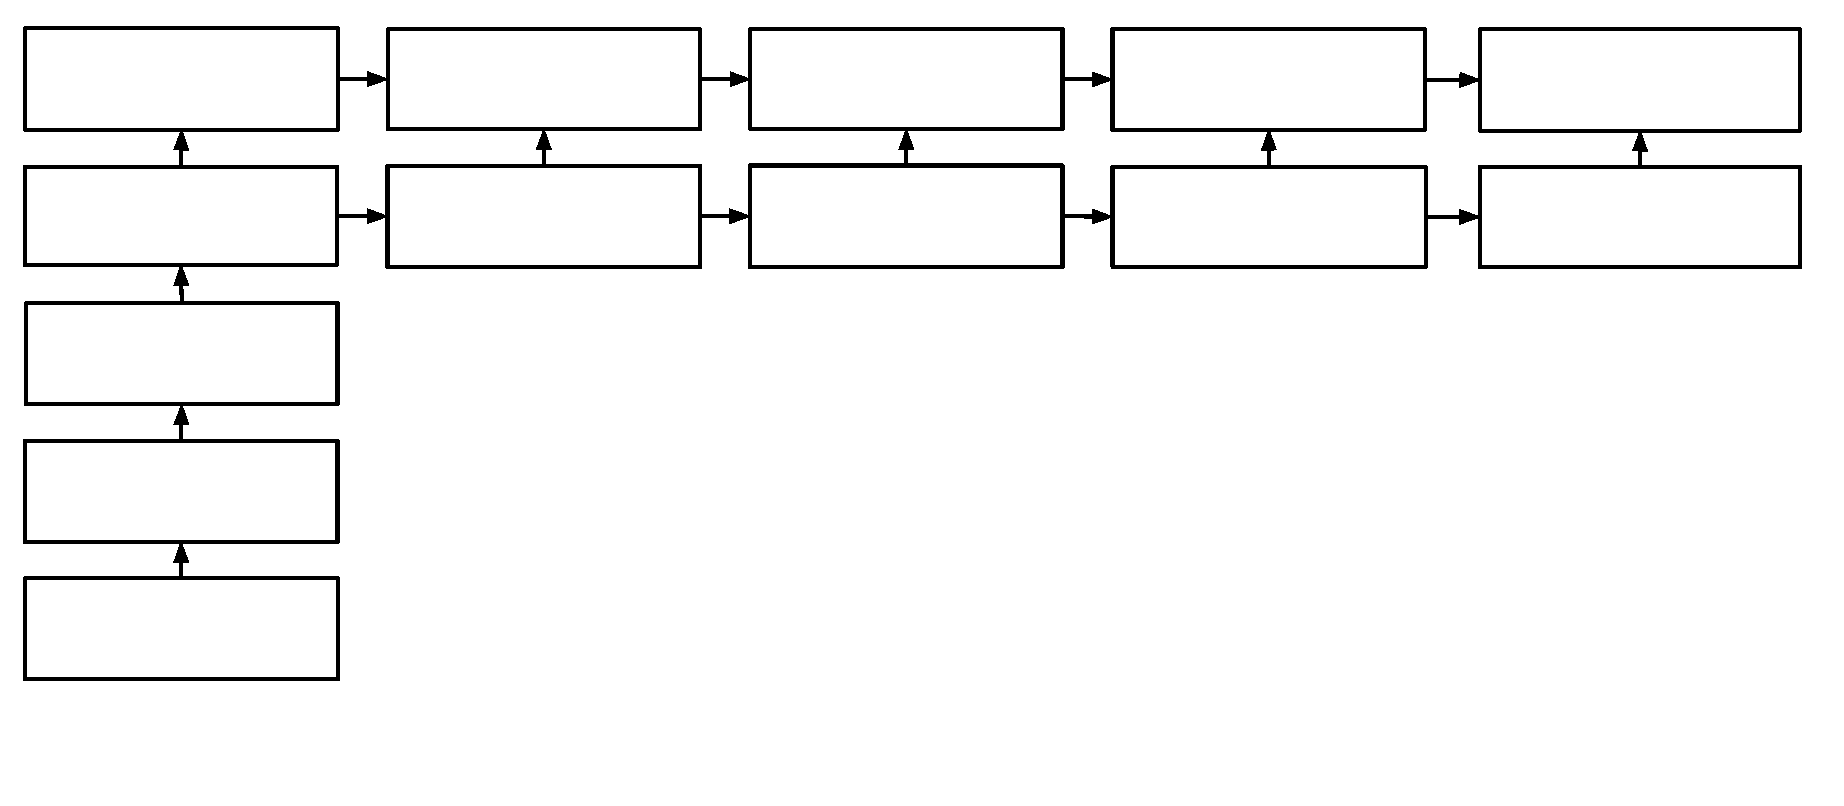
\includegraphics[width=\textwidth]{possible_pairs_of_states_of_parent_and_child_membrane}
    \caption{Possible pairs of states of parent and child membrane}
    \label{fig:possible_pairs_of_states_of_parent_and_child_membrane}
  \end{figure}

  \begin{figure}
    \def\svgwidth{\textwidth}
    \input{snapshot_of_all_membrane_states_while_simulating.pdf_tex}
    % 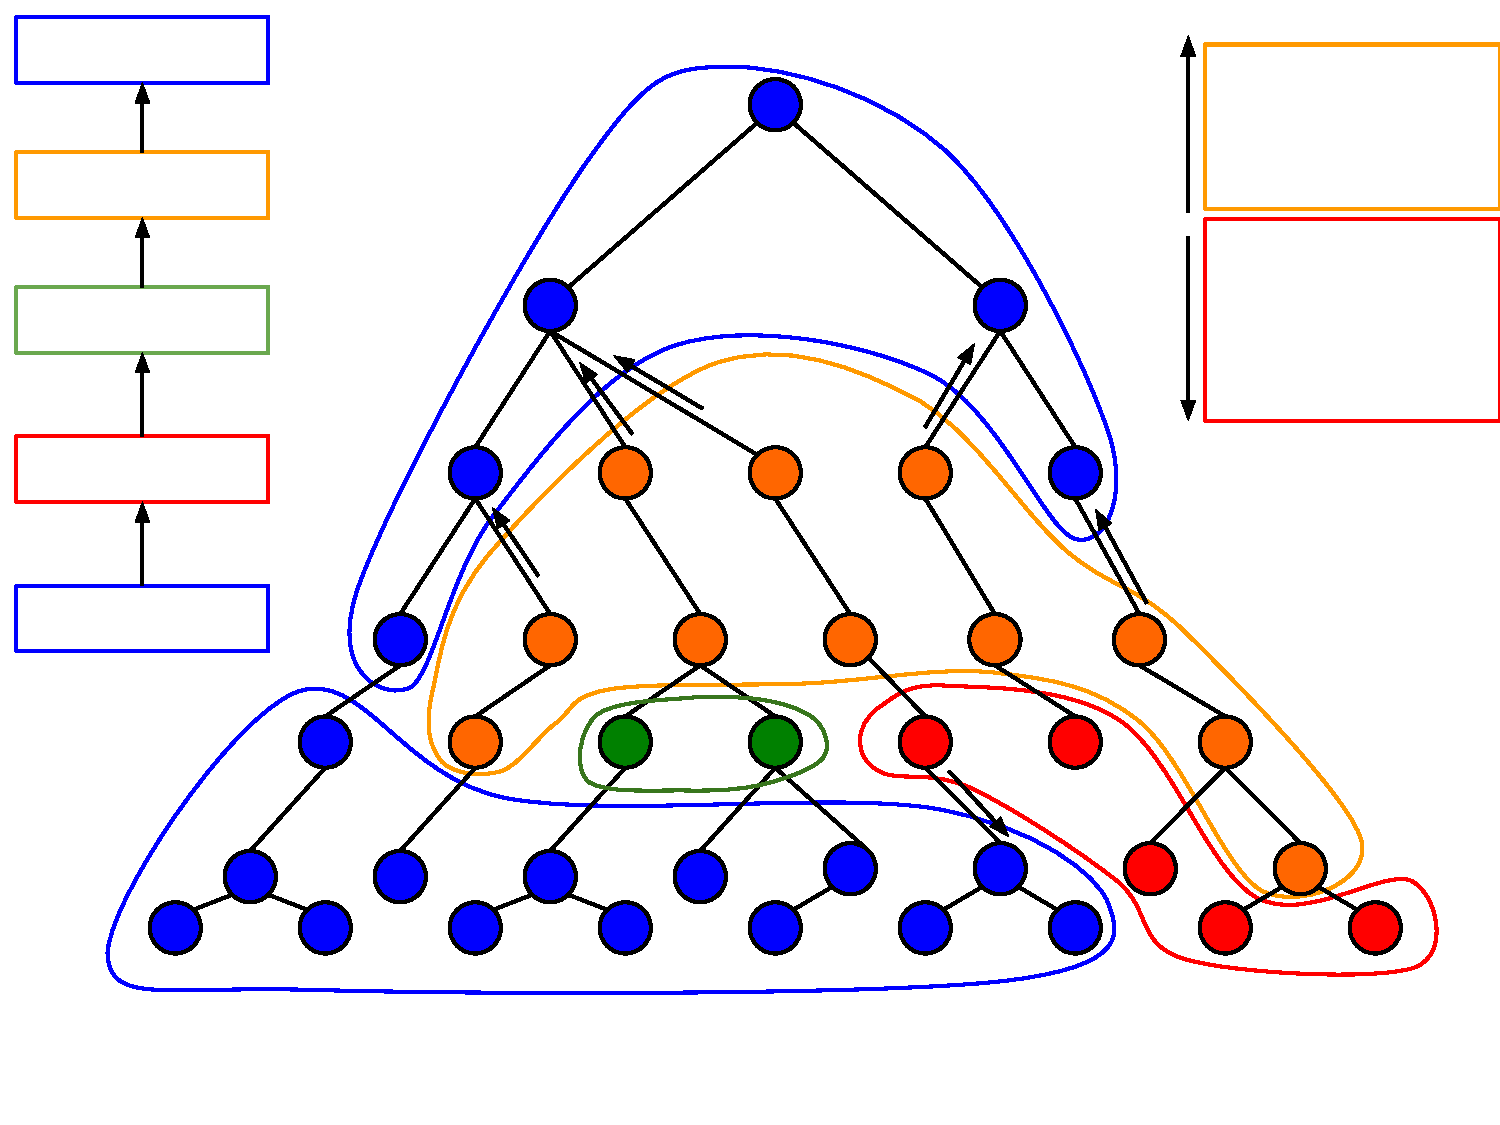
\includegraphics[width=\textwidth]{snapshot_of_all_membrane_states_while_simulating}
    \caption{Snapshot of all membrane states while simulating}
    \label{fig:snapshot_of_all_membrane_states_while_simulating}
  \end{figure}

  The pairs of possible phases of the parent and child membrane are shown in the figure \ref{fig:possible_pairs_of_states_of_parent_and_child_membrane} along with transitions between two consecutive global synchronizations - after the maximal parallel steps $i$ and $i+1$.

  In the figure \ref{fig:snapshot_of_all_membrane_states_while_simulating} the membrane structure is presented as a hierarchical structure. Every membrane is in one of four phases. It can be seen that the sending of the objects is performed in such phases that the receiving membrane is in either $RUN$ or $SYNCHRONIZE$ phase, so the received objects (marked $a^\prime$) does not interfere with rewriting.

  Another interesting idea can be seen in the figure \ref{fig:snapshot_of_all_membrane_states_while_simulating} that when a region is in the $SENDDOWN$ phase and objects are sent through the child membrane, the receiving region is in the $SYNCHRONIZE$ phase waiting for the $SYNCED$ signal, which will be sent to it when $SENDDOWN$ and $RESTORE$ phases finished.

  All membranes are nonempty during the simulation because at least the object representing the current phase is always present. By lemma~\ref{lemma:inhibitor_step} the rules with set of inhibitors can be simulated by single inhibitors.


\end{dokaz}




We have also reached this result in the accepting case by simulation of \index{Register machine} register machines.

% !TEX root = ../diz.tex
\begin{veta}
  Sequential P systems with cooperative rules and inhibitors can simulate register machines and thus equal $PsRE$.
\end{veta}


\begin{dokaz}
\label{proof:reg_by_inh}
  Suppose we have an $n$-register machine $M = (n,P,i,h)$. In our simulation we will have a membrane structure consisting of single membrane and the contents of register $j$ will be represented by the multiplicity of the object $a_j$.

  We will simulate the register machine by P system $(\Sigma, \mu, w, R)$, where:
  \begin{itemize}
    \item $\Sigma$ is an alphabet consisting of symbols that represent registers $a_1,\dots a_n$, instruction labels from the register machine $M$ and a halting symbol $\#$,
    \item $\mu$ is a membrane structure consisting of one single membrane,
    \item $w$ is initial contents of the membrane. It contains symbols for the input for the machine $a_i^{n_i}$ where $n_i$ is initial state of register with label $i$ and initial instruction label $e$.
    \item $R$ is a set of rules in the skin membrane.
  \end{itemize}
    
  For all instructions of type $(e : add(j), k, l)$ we will have rules:
  \begin{align*}
    e \rightarrow a_j|k\\
    e \rightarrow a_j|l.
  \end{align*}

  For all instructions of type $(e : sub(j), k, l)$ we will have rules:
  \begin{align*}
    e|a_j \rightarrow k\\
    e \rightarrow l|_{\neg a_j}.
  \end{align*}

  And finally halting rules:
  \begin{align*}
    h|a_j \rightarrow h|\#\text{~for all~}a\leq j\leq n,\\
    \# \rightarrow \#.
  \end{align*}

  For a configuration $(j, m_1, \dots, m_n)$ of the simulated register machine $M$ the skin membrane of the simulating P system contains a symbol $j$ and objects representing contents of registers $a_1^{m_1}, \dots, a_n^{m_n}$.

  When the halting instruction is reached, if there is an object present in the membrane, the hash symbol $\#$ is created and the rule $\# \rightarrow \#$ will be applicable forever as there is no rule to remove the symbol $\#$. If there is no object present, there is no rule to apply and computation will halt. It corresponds to the condition that all registers should be empty when halting. \qed
\end{dokaz}

\subsection{Concluding remarks} % (fold)
\label{sub:concluding_remarks_of_inhibitors}

Although these results are not very surprising as similar results already hold for Petri nets, which are equivalent to sequential P systems, the simulation of maximal parallel P system used in the proof for generating case is valuable not only for the universality, but also can be seen as a method of conversion between P systems in sequential manner and maximally parallel manner, which may be essential for future works on P systems and other multiset rewriting systems. Sequential variants are promising alternative to traditional maximal parallel variants and will be good subject for the further research. Future plans include research of other more restricted variants such as omitting cooperation in the rules or restricting the power of inhibitors.

% subsection concluding_remarks (end)
